\documentclass[a4paper,12pt]{exam}
\usepackage{graphicx}
\usepackage[document]{ragged2e}
 \usepackage[margin=1in]{geometry}
\usepackage{circuitikz}
\pagestyle{empty}
\usepackage{tikz}
\usepackage{multirow}
\usepackage{float}
\usepackage{amsmath}
\usepackage{multicol}
\usepackage{array}
\usepackage{enumitem}
\usepackage{setspace}
\usepackage{amssymb}

\usepackage{cite}
\usepackage{graphicx}
\usepackage{amsmath,amssymb,amsfonts,amsthm}
\usepackage{algorithmic}
\usepackage{graphicx}
\usepackage{textcomp}
\usepackage{xcolor}
\usepackage{txfonts}
\usepackage{listings}
\usepackage{enumitem}
\usepackage{mathtools}
\usepackage{gensymb}
\usepackage{comment}
\usepackage[breaklinks=true]{hyperref}
\usepackage{tkz-euclide} 
\usepackage{listings}
\usepackage{gvv}                                        
%\def\inputGnumericTable{}                                 
\usetikzlibrary{arrows.meta, positioning}
\usepackage{xparse}
\usepackage{color}                                            
\usepackage{array}                                            
\usepackage{longtable}                                       
\usepackage{calc}                                             
\usepackage{multirow}
\usepackage{multicol}
\usepackage{hhline}                                           
\usepackage{ifthen}                                           
\usepackage{lscape}
\usepackage{tabularx}
\usepackage{array}
\usepackage{float}
\newtheorem{theorem}{Theorem}[section]
\newtheorem{problem}{Problem}
\newtheorem{proposition}{Proposition}[section]
\newtheorem{lemma}{Lemma}[section]
\newtheorem{corollary}[theorem]{Corollary}
\newtheorem{example}{Example}[section]
\newtheorem{definition}[problem]{Definition}
\newcommand{\BEQA}{\begin{eqnarray}}
\newcommand{\EEQA}{\end{eqnarray}}
\usepackage{float}
%\newcommand{\define}{\stackrel{\triangle}{=}}
\theoremstyle{remark}
\usepackage{circuitikz}
\usepackage{tikz}
\usepackage{ragged2e}
\begin{document}

\raggedleft{\textbf{Electrical Engineering (EE)}}
\vspace{0.5cm}\\
\raggedright{\textbf{General Aptitude(GA)}}\\
\vspace{0.5cm}
\raggedright{\textbf{Q.1 - Q.5 Carry ONE mark Each}}
\begin{enumerate}
\item Rafi told Mary, "I am thinking of watching a film this weekend." 
The following reports on the above statement in indirect speech:\\ Rafi told Mary that 
\underline{\hspace{2cm}} of watching a film that weekend.\hfill{(GATE EE 2023)}
\begin{enumerate}
\begin{multicols}{4}
\item thought
\item is thinking
\item am thinking
\item was thinking
\end{multicols}
\end{enumerate}

\item Permit : \underline{\hspace{2cm}} :: Enforce : Relax \hfill{(GATE EE 2023)}\\
\brak{\text{By word meaning}}
\begin{enumerate}
\begin{multicols}{4}
\item Allow
\item Forbid
\item License
\item Reinforce
\end{multicols}
\end{enumerate}

\item Given a fair six-faced dice where the faces are labelled `1', `2', `3', `4', `5', and `6', what is the probability of getting a `1' on the first roll of the dice and a `4' on the second roll?\hfill{(GATE EE 2023)}
\begin{enumerate}
\begin{multicols}{4}
\item $\frac{1}{36}$
\item $\frac{1}{6}$
\item $\frac{5}{6}$
\item $\frac{1}{3}$
\end{multicols}
\end{enumerate}

\item A recent survey shows that $65\%$ of tobacco users were advised to stop consuming tobacco. 
The survey also shows that 3 out of 10 tobacco users attempted to stop using tobacco. \\
Based only on the information in the above passage, which one of the following options can be logically inferred with certainty?\hfill{(GATE EE 2023)}
\begin{enumerate}
\item A majority of tobacco users who were advised to stop consuming tobacco made an attempt to do so.
\item A majority of tobacco users who were advised to stop consuming tobacco did not attempt to do so.
\item Approximately $30\%$ of tobacco users successfully stopped consuming tobacco.
\item Approximately $65\%$ of tobacco users successfully stopped consuming tobacco.
\end{enumerate}

\item How many triangles are present in the given figure? \hfill{(GATE EE 2023)}
\begin{figure}[H]
    \centering
    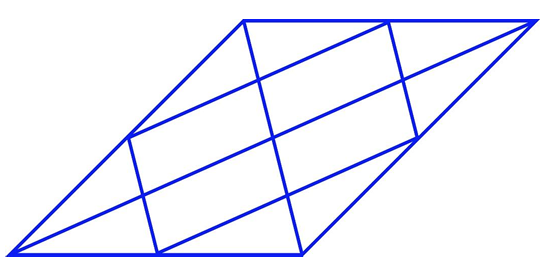
\includegraphics[width=0.3\columnwidth]{figs/Q 5.png}
    \caption{}
    \label{fig:placeholder}
\end{figure}


\begin{enumerate}
\begin{multicols}{4}
\item 12
\item 16
\item 20
\item 24
\end{multicols}
\end{enumerate}
\newpage
\item Students of all the departments of a college who have successfully completed the registration process are eligible to vote in the upcoming college elections. However, by the time the due date for registration was over, it was found that surprisingly none of the students from the Department of Human Sciences had completed the registration process. \\

Based only on the information provided above, which one of the following sets of statement\brak{\text{s}} can be logically inferred with certainty? \\
(i) All those students who would not be eligible to vote in the college elections would certainly belong to the Department of Human Sciences. \\
(ii) None of the students from departments other than Human Sciences failed to complete the registration process within the due time. \\
(iii) All the eligible voters would certainly be students who are not from the Department of Human Sciences.\hfill{(GATE EE 2023)}

\begin{enumerate}
\begin{multicols}{4}
\item (i) and (ii)
\item (i) and (iii)
\item only (i)
\item only (iii)
\end{multicols}
\end{enumerate}

\item Which one of the following options represents the given graph? \hfill{(GATE EE 2023)}
\begin{figure}[h]
    \centering
    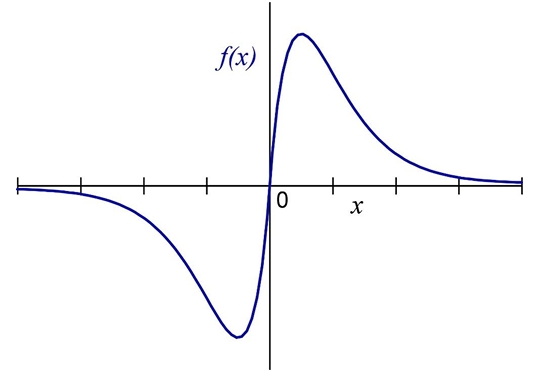
\includegraphics[width=0.4\columnwidth]{figs/Screenshot_17-8-2025_203313_.jpeg}
    \caption{}
    \label{fig:placeholder}
\end{figure}


\begin{enumerate}
\begin{multicols}{2}
\item $f(x) = x^2 2^{-|x|}$
\item $f(x) = x \, 2^{-|x|}$
\item $f(x) = |x| \, 2^{-x}$
\item $f(x) = x \, 2^{-x}$
\end{multicols}
\end{enumerate}

\item Which one of the options does NOT describe the passage below or follow from it? \\[0.5em]
We tend to think of cancer as a `modern' illness because its metaphors are so modern. It is a disease of overproduction, of sudden growth, a growth that is unstoppable, tipped into the abyss of no control. Modern cell biology encourages us to imagine the cell as a molecular machine. Cancer is that machine unable to quench its initial command \brak{\text{to grow}} and thus transform into an indestructible, self-propelled automaton. \hfill{(GATE EE 2023)}\\
\textit{[Adapted from The Emperor of All Maladies by Siddhartha Mukherjee]}

\begin{enumerate}
\item It is a reflection of why cancer seems so modern to most of us.
\item It tells us that modern cell biology uses and promotes metaphors of machinery.
\item Modern cell biology encourages metaphors of machinery, and cancer is often imagined as a machine.
\item Modern cell biology never uses figurative language, such as metaphors, to describe or explain anything.
\end{enumerate}
\newpage
\item The digit in the unit's place of the product $3^{999} \times 7^{1000}$ is \underline{\hspace{1cm}}. \hfill{(GATE EE 2023)}

\begin{enumerate}
\begin{multicols}{4}
\item 7
\item 1
\item 3
\item 9
\end{multicols}
\end{enumerate}

\item A square with sides of length $6 \ \text{cm}$ is given. The boundary of the shaded region is defined by two semi-circles whose diameters are the sides of the square, as shown. The area of the shaded region is \underline{\hspace{1cm}} $\text{cm}^2$. \hfill{(GATE EE 2023)}
\begin{figure}[h]
    \centering
    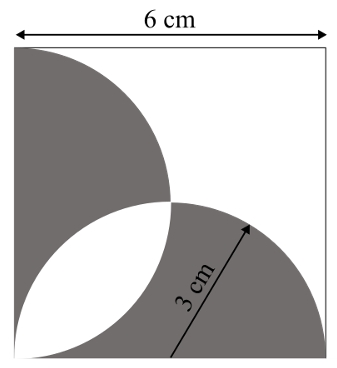
\includegraphics[width=0.5\columnwidth]{figs/Screenshot_17-8-2025_203345_.jpeg}
    \caption{}
    \label{fig:placeholder}
\end{figure}


\begin{enumerate}
\begin{multicols}{4}
\item $6\pi$
\item $18$
\item $20$
\item $9\pi$
\end{multicols}
\end{enumerate}

\raggedright{\textbf{Electrical Engineering}}\\
\vspace{0.5cm}
\raggedright{\textbf{Q.11 - Q.35 Carry ONE mark Each}}

\item For a given vector $\textbf{w} = \myvec{ 1 \\ 2 \\ 3 }$, the vector normal to the plane defined by $\textbf{w}^T \textbf{x} = 1$ is\hfill{(GATE EE 2023)}
\begin{multicols}{4}
\begin{enumerate}
    \item $\myvec{ -2 \\ -2 \\ 2 }$
    \item $\myvec{ 3 \\ 0 \\ -1 }$
    \item $\myvec{ 3 \\ 2 \\ 1 }$
    \item $\myvec{ 1 \\ 2 \\ 3 }$
\end{enumerate}
\end{multicols}
\newpage
\item For the block diagram shown in the figure, the transfer function  $\frac{Y(s)}{R(s)}$ is \hfill{(GATE EE 2023)}
\begin{figure}[H]
    \centering
    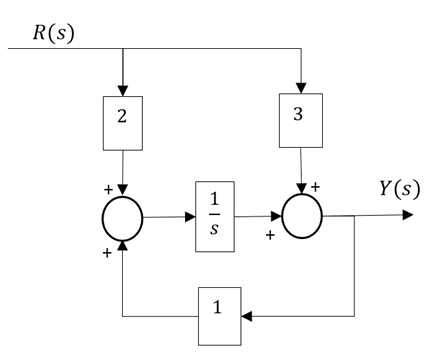
\includegraphics[width=0.5\columnwidth]{figs/Screenshot_17-8-2025_203411_.jpeg}
    \caption{}
    \label{fig:placeholder}
\end{figure}
\begin{multicols}{4}
\begin{enumerate}
    \item $\frac{2s+3}{s+1}$
    \item $\frac{3s+1}{s-1}$
    \item $\frac{s+1}{3s+2}$
    \item $\frac{3s+2}{s+1}$
\end{enumerate}
\end{multicols}
\item In the Nyquist plot of the open-loop transfer function

$G(s)H(s) = \frac{3s + 5}{s - 1}$
corresponding to the feedback loop, the infinite semi-circular arc of the Nyquist contour in $s$-plane is mapped into a point at\hfill{(GATE EE 2023)}
\begin{figure}[H]
    \centering
    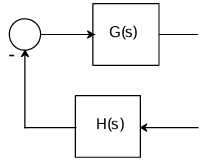
\includegraphics[width=0.4\columnwidth]{figs/Screenshot_17-8-2025_205719_.jpeg}
    \caption{Caption}
    \label{fig:placeholder}
\end{figure}
\begin{multicols}{4}
\begin{enumerate}
    \item $G(s)H(s) = \infty$
    \item $G(s)H(s) = 0$
    \item $G(s)H(s) = 3$
    \item $G(s)H(s) = -5$
\end{enumerate}
\end{multicols}
\newpage
\item Consider a unity-gain negative feedback system consisting of the plant $G(s)$ (given below) and a proportional-integral controller. Let the proportional gain and integral gain be 3 and 1, respectively. For a unit step reference input, the final values of the controller output and the plant output, respectively, are\hfill{(GATE EE 2023)}\\
$G(s) = \frac{1}{s-1}$

\begin{multicols}{4}
\begin{enumerate}
    \item $\infty,\, \infty$
    \item $1,\, 0$
    \item $1,\, -1$
    \item $-1,\, 1$
\end{enumerate}
\end{multicols}

\item The following columns present various modes of induction machine operation and the ranges of slip.\hfill{(GATE EE 2023)}
\begin{figure}[H]
    \centering
    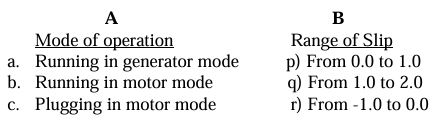
\includegraphics[width=0.9\columnwidth]{figs/Q 15.png}
\end{figure}

The correct matching between the elements in column \textbf{A} with those of column \textbf{B} is

\begin{multicols}{2}
\begin{enumerate}
    \item a-r, b-p, and c-q
    \item a-r, b-q, and c-p
    \item a-p, b-r, and c-q
    \item a-q, b-p, and c-r
\end{enumerate}
\end{multicols}
\item A 10-pole, 50 Hz, 240 V, single phase induction motor runs at 540 RPM while driving rated load. The frequency of induced rotor currents due to backward field is\hfill{(GATE EE 2023)}
\begin{multicols}{4}
\begin{enumerate}
    \item 100 Hz
    \item 95 Hz
    \item 10 Hz
    \item  5 Hz
\end{enumerate}
\end{multicols}
\item A continuous-time system that is initially at rest is described by
$
\frac{d y(t)}{dt} + 3y(t) = 2x(t),
$
where $x(t)$ is the input voltage and $y(t)$ is the output voltage. The impulse response of the system is\hfill{(GATE EE 2023)}

\begin{multicols}{4}
\begin{enumerate}
    \item $3e^{-2t}$
    \item $\dfrac{1}{3} e^{-2t} u(t)$
    \item $2e^{-3t} u(t)$
    \item $2e^{-3t}$
\end{enumerate}
\end{multicols}
\item The Fourier transform $X(\omega)$ of the signal $x(t)$ is given by\\
$
X(\omega) =1, \quad for \quad |\omega| < W_0$ \\
\hspace{1.3cm}0,$\quad for \quad |\omega| > W_0
$

Which one of the following statements is true?\hfill{(GATE EE 2023)}

\begin{multicols}{2}
\begin{enumerate}
    \item $x(t)$ tends to be an impulse as $W_0 \to \infty$.
    \item $x(0)$ decreases as $W_0$ increases.
    \item At $t = \dfrac{\pi}{2 W_0}$, $x(t) = -\dfrac{1}{\pi}$
    \item At $t = \dfrac{\pi}{2 W_0}$, $x(t) = \dfrac{1}{\pi}$
\end{enumerate}
\end{multicols}
\newpage
\item The Z-transform of a discrete signal $x[n]$ is
$
X(z) = \frac{4z}{\left(z - \frac{1}{5}\right)\left(z - \frac{2}{3}\right)\left(z - 3\right)} \quad \text{with ROC = } R.
$

Which one of the following statements is true?\hfill{(GATE EE 2023)}


\begin{enumerate}
    \item Discrete-time Fourier transform of $x[n]$ converges if $R$ is $|z| > 3$
    \item Discrete-time Fourier transform of $x[n]$ converges if $R$ is $\frac{2}{3} < |z| < 3$
    \item Discrete-time Fourier transform of $x[n]$ converges if $R$ is such that $x[n]$ is a left-sided sequence
    \item Discrete-time Fourier transform of $x[n]$ converges if $R$ is such that $x[n]$ is a right-sided sequence
\end{enumerate}

\item For the three-bus power system shown in the figure, the trip signals to the circuit breakers B$_1$ to B$_9$ are provided by overcurrent relays R$_1$ to R$_9$, respectively, some of which have directional properties also. The necessary condition for the system to be protected for short circuit fault at any part of the system between bus 1 and the R-L loads with isolation of minimum portion of the network using minimum number of directional relays is\hfill{(GATE EE 2023)}
\begin{figure}[H]
    \centering
    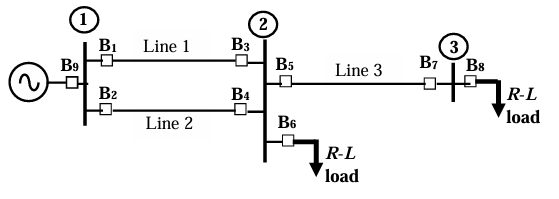
\includegraphics[width=0.5\columnwidth]{figs/Screenshot_17-8-2025_205732_.jpeg}
    \caption{}
    \label{fig:placeholder}
\end{figure}

\begin{enumerate}
    \item R$_3$ and R$_4$ are directional overcurrent relays blocking faults towards bus 2
    \item R$_3$ and R$_4$ are directional overcurrent relays blocking faults towards bus 2 and R$_7$ is directional overcurrent relay blocking faults towards bus 3
    \item R$_3$ and R$_4$ are directional overcurrent relays blocking faults towards Line 1 and Line 2, respectively, R$_7$ is directional overcurrent relay blocking faults towards Line 3 and R$_5$ is directional overcurrent relay blocking faults towards bus 2
    \item R$_3$ and R$_4$ are directional overcurrent relays blocking faults towards Line 1 and Line 2, respectively
\end{enumerate}
\newpage
\item The expressions of fuel cost of two thermal generating units as a function of the respective power generation $P_{G_1}$ and $P_{G_2}$ are given as\\
$
F_1(P_{G_1}) = 0.1aP_{G_1}^2 + 40P_{G_1} + 120~\text{Rs/hour} \quad 0~\text{MW} \leq P_{G_1} \leq 350~\text{MW}
$
$
F_2(P_{G_2}) = 0.2P_{G_2}^2 + 30P_{G_2} + 100~\text{Rs/hour} \quad 0~\text{MW} \leq P_{G_2} \leq 300~\text{MW}
$\\

where $a$ is a constant. For a given value of $a$, optimal dispatch requires the total load of 290 MW to be shared as $P_{G_1} = 175~MW$ and $P_{G_2} = 115~MW$. With the load remaining unchanged, the value of $a$ is increased by 10\% and optimal dispatch is carried out. The changes in $P_{G_1}$ and the total cost of generation, $F$ ($= F_1 + F_2$) in Rs/hour will be as follows\hfill{(GATE EE 2023)}

\begin{multicols}{2}
\begin{enumerate}
    \item $P_{G_1}$ will decrease and $F$ will increase
    \item Both $P_{G_1}$ and $F$ will increase
    \item $P_{G_1}$ will increase and $F$ will decrease
    \item Both $P_{G_1}$ and $F$ will decrease
\end{enumerate}
\end{multicols}

\item The four stator conductors (A, A$'$, B and B$'$) of a rotating machine are carrying DC currents of the same value, the directions of which are shown in the figure (i). The rotor coils a-a$'$ and b-b$'$ are formed by connecting the back ends of conductors ‘a’ and ‘a$'$’ and ‘b’ and ‘b$'$’, respectively, as shown in figure (ii). The e.m.f. induced in coil a-a$'$ and coil b-b$'$ are denoted by $E_{a-a'}$ and $E_{b-b'}$, respectively. If the rotor is rotated at uniform angular speed $\omega$ rad/s in the clockwise direction then which of the following correctly describes the $E_{a-a'}$ and $E_{b-b'}$?\hfill{(GATE EE 2023)}
\begin{figure}[H]
    \centering
    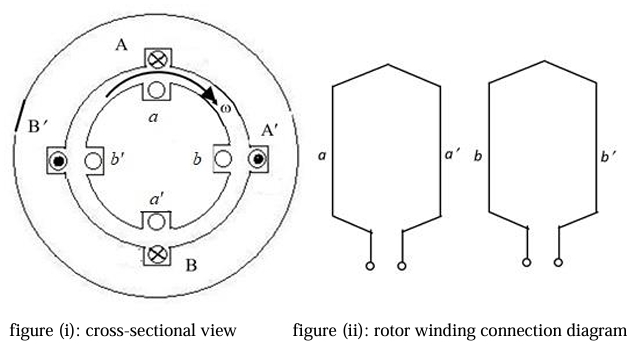
\includegraphics[width=0.85\columnwidth]{figs/Screenshot_17-8-2025_205746_.jpeg}
    \caption{}
    \label{fig:placeholder}
\end{figure}
\begin{multicols}{4}
\begin{enumerate}
    \item $E_{a-a'}$ and $E_{b-b'}$ have finite magnitudes and are in the same phase
    \item $E_{a-a'}$ and $E_{b-b'}$ have finite magnitudes with $E_{b-b'}$ leading $E_{a-a'}$
    \item $E_{a-a'}$ and $E_{b-b'}$ have finite magnitudes with $E_{a-a'}$ leading $E_{b-b'}$
    \item $E_{a-a'} = E_{b-b'} = 0$
\end{enumerate}
\end{multicols}
\newpage
\item The chopper circuit shown in figure (i) feeds power to a 5~A DC constant current source. The switching frequency of the chopper is 100~kHz. All the components can be assumed to be ideal. The gate signals of switches $S_1$ and $S_2$ are shown in figure (ii). Average voltage across the 5~A current source is\hfill{(GATE EE 2023)}
\begin{figure}[H]
    \centering
    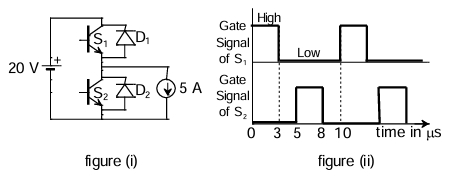
\includegraphics[width=0.8\columnwidth]{figs/Screenshot_17-8-2025_205755_.jpeg}
    \caption{}
    \label{fig:placeholder}
\end{figure}
\begin{multicols}{4}
\begin{enumerate}
    \item 10V
    \item 6V
    \item 12V
    \item 20V
\end{enumerate}
\end{multicols}

\item In the figure, the vectors $\textbf{u}$ and $\textbf{v}$ are related as: $\textbf{A}\textbf{u} = \textbf{v}$ by a transformation matrix $\textbf{A}$. The correct choice of $\textbf{A}$ is\hfill{(GATE EE 2023)}

\begin{figure}[H]
    \centering
    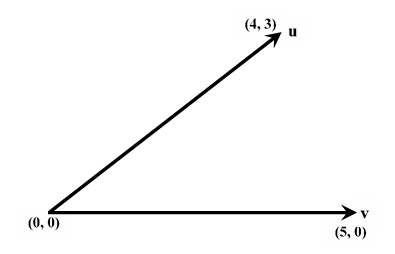
\includegraphics[width=0.5\columnwidth]{figs/Q 24.png}
    \caption{}
    \label{fig:placeholder}
\end{figure}
\begin{multicols}{4}
\begin{enumerate}
    \item $ \myvec{
\dfrac{4}{5} & \dfrac{3}{5} \\
\dfrac{3}{5} & -\dfrac{4}{5}
}$
    \item $ \myvec{
\dfrac{4}{5} & -\dfrac{3}{5} \\
\dfrac{3}{5} & \dfrac{4}{5}
}$
    \item $ \myvec{
\dfrac{4}{5} & \dfrac{3}{5} \\
\dfrac{3}{5} & \dfrac{4}{5}
}$
    \item $ \myvec{
\dfrac{4}{5} & -\dfrac{3}{5} \\
\dfrac{3}{5} & -\dfrac{4}{5}
}$
\end{enumerate}
\end{multicols}
\newpage

\item One million random numbers are generated from a statistically stationary process with a Gaussian distribution with mean zero and standard deviation $\sigma_0$. 

The $\sigma_0$ is estimated by randomly drawing out 10,000 numbers of samples ($x_n$). The estimates $\hat{\sigma}_1$, $\hat{\sigma}_2$ are computed in the following two ways.
$
\hat{\sigma}_1^2 = \frac{1}{10000} \sum_{n=1}^{10000} x_n^2
\qquad
\hat{\sigma}_2^2 = \frac{1}{9999} \sum_{n=1}^{10000} x_n^2
$

Which of the following statements is true?\hfill{(GATE EE 2023)}
\begin{multicols}{4}
\begin{enumerate}
    \item $E(\hat{\sigma}_2^2) = \sigma_0^2$
    \item $E(\hat{\sigma}_2) = \sigma_0$
    \item $E(\hat{\sigma}_1^2) = \sigma_0^2$
    \item $E(\hat{\sigma}_1) = E(\hat{\sigma}_2)$
\end{enumerate}
\end{multicols}
\item A semiconductor switch needs to block voltage $V$ of only one polarity ($V > 0$) during OFF state as shown in figure (i) and carry current in both directions during ON state as shown in figure (ii). Which of the following switch combination(s) will realize the same?\hfill{(GATE EE 2023)}
\begin{figure}[H]
    \centering
    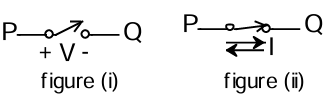
\includegraphics[width=0.4\columnwidth]{figs/Q 26.png}
    \caption{}
    \label{fig:placeholder}
\end{figure}


\begin{multicols}{2}
\begin{enumerate}
    \item \begin{figure}[H]
    \centering
    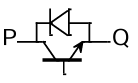
\includegraphics[width=0.5\columnwidth]{figs/Q 26 1.png}
    
\end{figure}
    \item \begin{figure}[H]
    \centering
    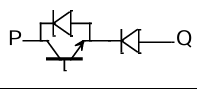
\includegraphics[width=0.5\columnwidth]{figs/Q 26 2.png}
    
\end{figure}
    \item \begin{figure}[H]
    \centering
    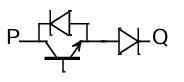
\includegraphics[width=0.5\columnwidth]{figs/Q 26 3.png}
    
\end{figure}
    \item \begin{figure}[H]
    \centering
    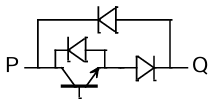
\includegraphics[width=0.5\columnwidth]{figs/Q 26 4.png}
   
\end{figure}
\end{enumerate}
\end{multicols}
\item Which of the following statement(s) is/are true?\hfill{(GATE EE 2023)}

\begin{enumerate}
    \item If an LTI system is causal, it is stable
    \item A discrete time LTI system is causal if and only if its response to a step input $u[n]$ is $0$ for $n < 0$
    \item If a discrete time LTI system has an impulse response $h[n]$ of finite duration the system is stable
    \item If the impulse response $0 < |h[n]| < 1$ for all $n$, then the LTI system is stable.
\end{enumerate}
\newpage
\item  The bus admittance ($Y_{bus}$) matrix of a 3-bus power system is given below.

\quad\quad\quad\quad 1 \quad\quad 2 \quad\quad 3\\
\hspace{1.1cm}
$
\myvec{
    -j15 & j10 & j5 \\
    j10 & -j13.5 & j4 \\
    j5 & j4 & -j8
}
$


Considering that there is no shunt inductor connected to any of the buses, which of the following can NOT be true?\hfill{(GATE EE 2023)}
\begin{enumerate}
    \item Line charging capacitor of finite value is present in all three lines
    \item Line charging capacitor of finite value is present in line 2-3 only
    \item Line charging capacitor of finite value is present in line 2-3 only and shunt capacitor of finite value is present in bus 1 only
    \item Line charging capacitor of finite value is present in line 2-3 only and shunt capacitor of finite value is present in bus 3 only
\end{enumerate}

\item The value of parameters of the circuit shown in the figure are
$
R_1 = 2\Omega, \; R_2 = 2\Omega, \; R_3 = 3\Omega, \; L = 10mH, \; C = 100\mu F
$

For time $t < 0$, the circuit is at steady state with the switch `K' in closed condition. If the switch is opened at $t = 0$, the value of the voltage across the inductor ($V_L$) at $t = 0^+$ in Volts is \rule{2cm}{0.15mm} (Round off to 1 decimal place).\hfill{(GATE EE 2023)}
\begin{figure}[H]
    \centering
    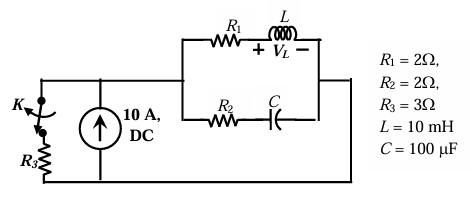
\includegraphics[width=0.5\columnwidth]{figs/Q 29.png}
    \caption{}
    \label{fig:placeholder}
\end{figure}

\item A separately excited DC motor rated 400~V, 15~A, 1500~RPM drives a constant torque load at rated speed operating from 400~V DC supply drawing rated current. The armature resistance is 1.2~$\Omega$. If the supply voltage drops by 10\% with field current unaltered then the resultant speed of the motor in RPM is \rule{2cm}{0.15mm} (Round off to the nearest integer).\hfill{(GATE EE 2023)}

\item For the signals $x(t)$ and $y(t)$ shown in the figure, $z(t) = x(t) * y(t)$ is maximum at $t = T_1$. Then $T_1$ in seconds is \rule{2cm}{0.15mm} (Round off to the nearest integer).\hfill{(GATE EE 2023)}
\newpage
\begin{figure}[H]
    \centering
    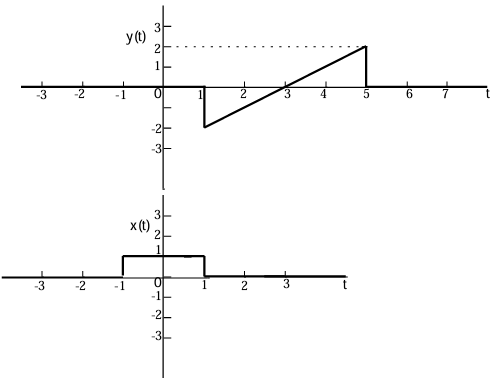
\includegraphics[width=0.5\columnwidth]{figs/Q 31.png}
    \caption{}
    \label{fig:placeholder}
\end{figure}


\item For the circuit shown in the figure, $V_1 = 8$~V, DC and $I_1 = 8$~A, DC. The voltage $V_{ab}$ in Volts is \rule{2cm}{0.15mm} (Round off to 1 decimal place).\hfill{(GATE EE 2023)}
\begin{figure}[H]
    \centering
    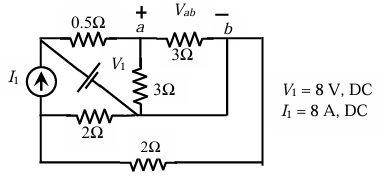
\includegraphics[width=0.5\columnwidth]{figs/Q 32.png}
    \caption{}
    \label{fig:placeholder}
\end{figure}

\item A 50 Hz, 275 kV line of length 400 km has the following parameters:

\begin{align*}
\text{Resistance, } & R = 0.035~\Omega/\text{km}; \\
\text{Inductance, } & L = 1~\text{mH}/\text{km}; \\
\text{Capacitance, } & C = 0.01~\mu\text{F}/\text{km};
\end{align*}

The line is represented by the nominal-$\pi$ model. With the magnitudes of the sending end and the receiving end voltages of the line (denoted by $V_S$ and $V_R$, respectively) maintained at 275 kV, the phase angle difference ($\theta$) between $V_S$ and $V_R$ required for maximum possible active power to be delivered to the receiving end, in degree is \rule{2cm}{0.15mm} (Round off to 2 decimal places).\hfill{(GATE EE 2023)}

\item In the following differential equation, the numerically obtained value of $y(t)$, at $t=1$, is \rule{2cm}{0.15mm} (Round off to 2 decimal places).
\hfill{(GATE EE 2023)}\\
$
\frac{dy}{dt} = \frac{e^{-\alpha t}}{2 + \alpha t}, \qquad \alpha = 0.01 \text{ and } y(0) = 0
$

\item Three points in the $x$-$y$ plane are $(-1,~0.8)$, $(0,~2.2)$ and $(1,~2.8)$. The value of the slope of the best fit straight line in the least square sense is \rule{2cm}{0.15mm} (Round off to 2 decimal places).\hfill{(GATE EE 2023)}
\newpage
\item The magnitude and phase plots of an LTI system are shown in the figure. The 
transfer function of the system is \hfill{(GATE EE 2023)}
\begin{figure}[H]
    \centering
    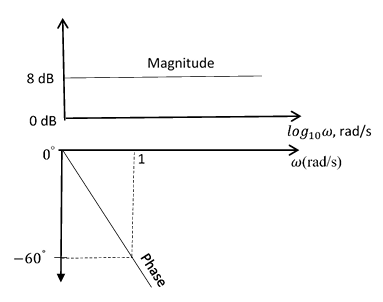
\includegraphics[width=0.5\columnwidth]{figs/Q 36.png}
    \caption{}
    \label{fig:placeholder}
\end{figure}

\begin{multicols}{4}
\begin{enumerate}
    \item $2.51 e^{-0.032s}$
    \item $\frac{e^{-2.514s}}{s+1}$
    \item $1.04 e^{-2.514s}$
    \item $2.51 e^{-1.047s}$
\end{enumerate}
\end{multicols}
\item Consider the OP AMP based circuit shown in the figure. Ignore the conduction 
drops of diodes $ D_{1}$ and$ D_{2}$. All the components are ideal and the breakdown voltage of the Zener is 5 V. Which of the following statements is true? \hfill{(GATE EE 2023)}
\begin{figure}[H]
    \centering
    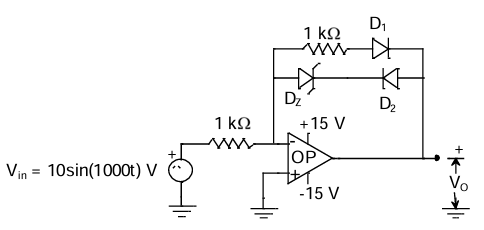
\includegraphics[width=0.5\columnwidth]{figs/Q 37.png}
    \caption{}
    \label{fig:placeholder}
\end{figure}
\begin{enumerate}
    \item The maximum and minimum values of the output voltage $V_{0}$ are +15 V and -10 V, respectively.
    \item The maximum and minimum values of the output voltage $V_{0}$ are +5 V and -15 V, 
respectively. 
    \item The maximum and minimum values of the output voltage $V_{0}$ are +10 V and -5 V, 
respectively. 
    \item The maximum and minimum values of the output voltage $V_{0}$ are +10 V and -5 V, 
respectively. 
\end{enumerate}
\newpage
\item Consider a lead compensator of the form\hfill{(GATE EE 2023)}

$
K(s) = \frac{1 + \frac{s}{a}}{1 + \frac{s}{\beta a}},\ \beta > 1,\, \alpha > 0
$

The frequency at which this compensator produces maximum phase lead is 4~rad/s.
At this frequency, the gain amplification provided by the controller, assuming asymptotic Bode-magnitude plot of $K(s)$, is 6~dB. The values of $\alpha, \beta$, respectively, are
\begin{multicols}{4}
\begin{enumerate}
    \item 1,16
    \item 2,4
    \item 3,5
    \item 2.66, 2.25
\end{enumerate}
\end{multicols}
\item A 3-phase, star-connected, balanced load is supplied from a 3-phase, 400 V (rms), 
balanced voltage source with phase sequence R-Y-B, as shown in the figure. If the 
wattmeter reading is $-400 W$ and the line current is $I_{R}=2 $A (rms), then the power 
factor of the load per phase is \hfill{(GATE EE 2023)}
\begin{figure}[H]
    \centering
    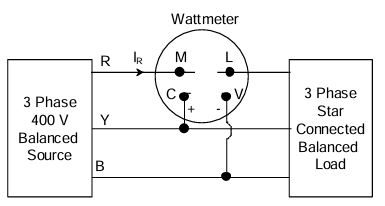
\includegraphics[width=0.5\columnwidth]{figs/Q 39.png}
    \caption{}
    \label{fig:placeholder}
\end{figure}
\begin{multicols}{4}
\begin{enumerate}
    \item Unity
    \item 0.5 leading
    \item 0.866 leading
    \item 0.707 lagging
\end{enumerate}
\end{multicols}
\item An 8 bit ADC converts analog voltage in the range of 0 to +5 V to the corresponding 
digital code as per the conversion characteristics shown in figure.  
For  $V_{in}=1.9922$ , which of the following digital output, given in hex, is true ? \hfill{(GATE EE 2023)}

\begin{figure}[H]
    \centering
    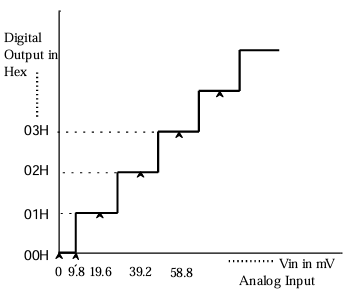
\includegraphics[width=0.4\columnwidth]{figs/Q 40.png}
    \caption{}
    \label{fig:placeholder}
\end{figure}
\begin{multicols}{4}
\begin{enumerate}
    \item 64H
    \item 65H
    \item 66H
    \item 67H
\end{enumerate}
\end{multicols}
\newpage
\item The three-bus power system shown in the figure has one alternator connected to bus 2 which supplies 200~MW and 40~MVAr power. Bus~3 is infinite bus having a voltage of magnitude $|V_3| = 1.0$~p.u. and angle of $-15^\circ$. A variable current source, $|I|\angle \phi$ is connected at bus~1 and controlled such that the magnitude of the bus~1 voltage is maintained at 1.05~p.u. and the phase angle of the source current, $\phi = \theta_1 \pm \frac{\pi}{2}$, where $\theta_1$ is the phase angle of the bus~1 voltage. The three buses can be categorized for load flow analysis as\hfill{(GATE EE 2023)}
\begin{figure}[H]
    \centering
    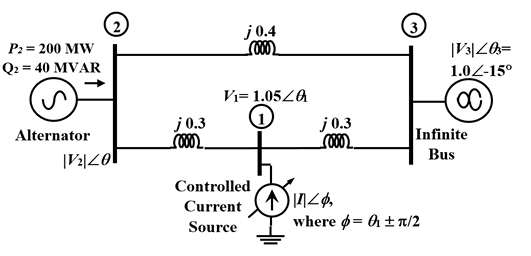
\includegraphics[width=0.8\columnwidth]{figs/Q 41.png}
    \caption{}
    \label{fig:placeholder}
\end{figure}

\begin{multicols}{2}
\begin{enumerate}
    \item Bus 1\quad Slack bus\\
Bus 2\quad$P-|V|$ bus\\
Bus 3\quad$P-Q$ bus
    \item Bus 1\quad$P-|V|$ bus\\
Bus 2\quad$P-|V|$ bus\\
Bus 3\quad Slack bus
    \item Bus 1\quad $P-Q$ bus\\
Bus 2\quad $P-Q$ bus\\
Bus 3\quad  Slack bus

    \item Bus 1\quad $P-|V|$ bus\\
Bus 2\quad $P-Q$ bus\\
Bus 3\quad Slack bus

\end{enumerate}
\end{multicols}

\item Consider the following equation in a 2-D real-space.

$
|x_1|^p + |x_2|^p = 1 \quad \text{for } p > 0
$

Which of the following statement(s) is/are true.\hfill{(GATE EE 2023)}
\begin{enumerate}
    \item When $p=2$, the area enclosed by the curve is $\pi$.
    \item When $p$ tends to $\infty$, the area enclosed by the curve tends to $4$.
    \item When $p$ tends to $0$, the area enclosed by the curve is $1$.
    \item When $p=1$, the area enclosed by the curve is $2$.
\end{enumerate}
\newpage

\item
In the figure, the electric field $\textbf{E}$ and the magnetic field $\textbf{B}$ point to $x$ and $z$ directions, respectively, and have constant magnitudes. A positive charge `$q$' is released from rest at the origin. Which of the following statement(s) is/are true.\hfill{(GATE EE 2023)}

\begin{figure}[H]
    \centering
    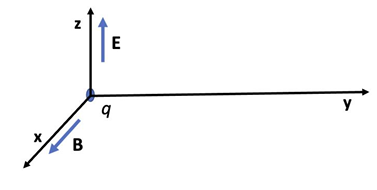
\includegraphics[width=0.5\columnwidth]{figs/Q 43.png}
    \caption{}
    \label{fig:placeholder}
\end{figure}
\begin{enumerate}
    \item The charge will move in the direction of $z$ with constant velocity.
    \item The charge will always move on the \textbf{y-z} plane only.
    \item The trajectory of the charge will be a circle.
    \item The charge will progress in the direction of \textbf{y}.
\end{enumerate}
\item All the elements in the circuit shown in the following figure are ideal. Which of the following statements is/are true? \hfill{(GATE EE 2023)}

\begin{enumerate}
    \item When switch $S$ is ON, both $D_1$ and $D_2$ conduct and $D_3$ is reverse biased
    \item When switch $S$ is ON, $D_1$ conducts and both $D_2$ and $D_3$ are reverse biased
    \item When switch $S$ is OFF, $D_1$ is reverse biased and both $D_2$ and $D_3$ conduct
    \item When switch $S$ is OFF, $D_1$ conducts, $D_2$ is reverse biased and $D_3$ conducts
\end{enumerate}
\item The expected number of trials for first occurrence of a “head” in a biased coin is 
known to be 4. The probability of first occurrence of a “head” in the second trial is \rule{2cm}{0.15mm}
 (Round off to 3 decimal places). \hfill{(GATE EE 2023)}

 \item Consider the state-space description of an LTI system with matrices\hfill{(GATE EE 2023)}
$
A = \myvec{ 0 & 1 \\ -1 & -2 }, \quad
B = \myvec{ 0 \\ 1 }, \quad
C = \myvec{ 3 & -2 }, \quad
D = 1
$\\
For the input, $\sin(\omega t)$, $\omega > 0$, the value of $\omega$ for which the steady-state output of the system will be zero, is \underline{\hspace{2cm}} (Round off to the nearest integer).

\item A three-phase synchronous motor with synchronous impedance of $0.1 + j0.3$ per unit per phase has a static stability limit of 2.5 per unit. The corresponding excitation voltage in per unit is \underline{\hspace{2cm}} (Round off to 2 decimal places).\hfill{(GATE EE 2023)}

\item A three-phase 415~V, 50~Hz, 6-pole, 960~RPM, 4~HP squirrel cage induction motor drives a constant torque load at rated speed operating from rated supply and delivering rated output. If the supply voltage and frequency are reduced by 20\%, the resultant speed of the motor in RPM (neglecting the stator leakage impedance and rotational losses) is \underline{\hspace{2cm}} (Round off to the nearest integer).\hfill{(GATE EE 2023)}
\newpage

\item The period of the discrete-time signal $x[n]$ described by the equation below is $N = \underline{\hspace{2cm}}$ (Round off to the nearest integer).\hfill{(GATE EE 2023)}
$
x[n] = 1 + 3 \sin \left( \frac{15\pi}{8} n + \frac{3\pi}{4} \right) - 5 \sin \left( \frac{\pi}{3} n - \frac{\pi}{4} \right)
$

\item The discrete-time Fourier transform of a signal $x[n]$ is $X(\Omega) = (1 + \cos \Omega) e^{-j\Omega}$.\\
Consider that $x_p[n]$ is a periodic signal of period $N=5$ such that
$
x_p[n] = 
\begin{cases}
x[n], & \text{for } n=0,1,2 \\
0, & \text{for } n=3,4 \\
\end{cases}
$
Note that $x_p[n] = \sum_{k=0}^{N-1} a_k e^{j \frac{2\pi}{N} k n}$. The magnitude of the Fourier series coefficient $a_3$ is \underline{\hspace{2cm}} (Round off to 3 decimal places).\hfill{(GATE EE 2023)}
\item For the circuit shown, if i = $\sin 1000t$, the instantaneous value of the Thevenin’s 
equivalent voltage (in Volts) across the terminals a-b at time t = 5 ms is \underline{\hspace{2cm}}
(Round off to 2 decimal places). \hfill{(GATE EE 2023)}

\begin{figure}[H]
    \centering
    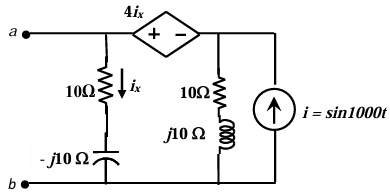
\includegraphics[width=0.5 \columnwidth]{figs/Q 51.png}
    \caption{}
    \label{fig:placeholder}
\end{figure}

 \item The admittance parameters of the passive resistive two-port network shown in the 
figure are 
$y_{11}=5S, y_{22}=1 S, y_{12}=y_{21} = -2.5 S $
The power delivered to the load resistor RL in Watt is  (Round off to 2 
decimal places).\hfill{(GATE EE 2023)}
\begin{figure}[H]
    \centering
    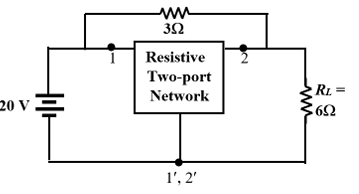
\includegraphics[width=0.5 \columnwidth]{figs/Q 52.png}
    \caption{}
    \label{fig:placeholder}
\end{figure}
\item When the winding $c$-$d$ of the single-phase, 50~Hz, two winding transformer is supplied from an AC current source of frequency 50~Hz, the rated voltage of 200~V (rms), 50~Hz is obtained at the open-circuited terminals $a$-$b$. The cross sectional area of the core is $5000 mm^2$ and the average core length traversed by the mutual flux is $500 mm$. The maximum allowable flux density in the core is $B_{\text{max}} = 1 Wb/m^2$ and the relative permeability of the core material is $5000$. The leakage impedance of the winding $a$-$b$ and winding $c$-$d$ at 50~Hz are $(5 + j100\pi \times 0.16)~\Omega$ and $(11.25 + j100\pi \times 0.36)~\Omega$, respectively. Considering the magnetizing characteristics to be linear and neglecting core loss, the self-inductance of the winding $a$-$b$ in millihenry is \underline{\hspace{2cm}}. (Round off to 1 decimal place).\hfill{(GATE EE 2023)}
\begin{figure}[H]
    \centering
    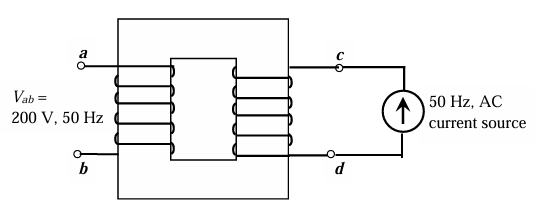
\includegraphics[width=0.5 \columnwidth]{figs/Q 53.png}
    \caption{}
    \label{fig:placeholder}
\end{figure}

\item The circuit shown in the figure is initially in the steady state with the switch $K$ in open condition and $\overline{K}$ in closed condition. The switch $K$ is closed and $\overline{K}$ is opened simultaneously at the instant $t = t_1$, where $t_1 > 0$. The minimum value of $t_1$ in milliseconds, such that there is no transient in the voltage across the 100~$\mu$F capacitor, is \underline{\hspace{2cm}}. (Round off to 2 decimal places).\hfill{(GATE EE 2023)}
\begin{figure}[H]
    \centering
    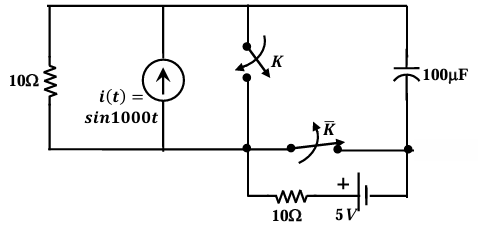
\includegraphics[width=0.5 \columnwidth]{figs/Q 54.png}
    \caption{}
    \label{fig:placeholder}
\end{figure}
 \item The circuit shown in the figure has reached steady state with thyristor ‘T’ in OFF 
condition. Assume that the latching and holding currents of the thyristor are zero. 
The thyristor is turned ON at$ t = 0$ sec. The duration in microseconds for which the 
thyristor would conduct, before it turns off, is \underline{\hspace{2cm}}(Round off to 2 decimal 
places).\hfill{(GATE EE 2023)}
\begin{figure}[H]
    \centering
    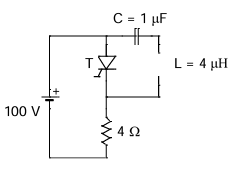
\includegraphics[width=0.4\columnwidth]{figs/Q 55.png}
    \caption{}
    \label{fig:placeholder}
\end{figure}
\item Neglecting the delays due to the logic gates in the circuit shown in figure, the 
decimal equivalent of the binary sequence [ABCD] of initial logic states, which 
will not change with clock, is \underline{\hspace{2cm}}\hfill{(GATE EE 2023)}
\begin{figure}[H]
    \centering
    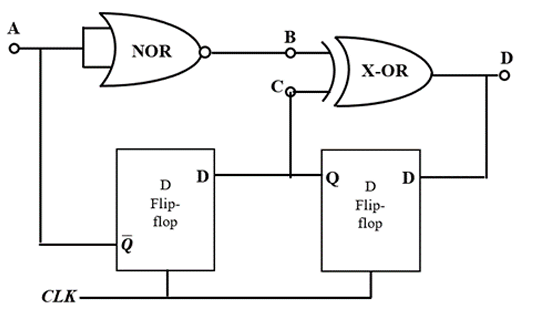
\includegraphics[width=0.7\columnwidth]{figs/Q 56.png}
    \caption{}
    \label{fig:placeholder}
\end{figure}
\item In a given 8-bit general purpose micro-controller there are following flags.\\

 C-Carry,  A-Auxiliary Carry,  O-Overflow flag,  P-Parity (0 for even, 1 for odd)\\

R0 and R1 are the two general purpose registers of the micro-controller.\\

After execution of the following instructions, the decimal equivalent of the binary sequence of the flag pattern [CAOP] will be \underline{\hspace{3cm}}.\hfill{(GATE EE 2023)}\\
MOV R0, +0x60\\
MOV R1, +0x46\\
ADD R0, R1

\item The single phase rectifier consisting of three thyristors $T_1$, $T_2$, $T_3$ and a diode $D_1$ feed power to a 10~A constant current load. $T_1$ and $T_3$ are fired at $\alpha = 60^\circ$ and $T_2$ is fired at $\alpha = 240^\circ$. The reference for $\alpha$ is the positive zero crossing of $V_{in}$. The average voltage $V_O$ across the load in volts is \underline{\hspace{3cm}} (Round off to 2 decimal places).\hfill{(GATE EE 2023)}
\begin{figure}[H]
    \centering
    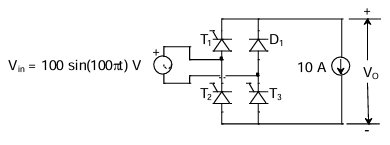
\includegraphics[width=0.7\columnwidth]{figs/Q 58.png}
    \caption{}
    \label{fig:placeholder}
\end{figure}
\newpage
\item The Zener diode in circuit has a breakdown voltage of 5~V. The current gain $\beta$ of the transistor in the active region in 99. Ignore base-emitter voltage drop $V_{BE}$. The current through the $20~\Omega$ resistance in milliamperes is \underline{\hspace{3cm}} (Round off to 2 decimal places).\hfill{(GATE EE 2023)}
\begin{figure}[H]
    \centering
    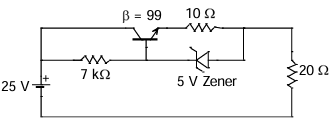
\includegraphics[width=0.5\columnwidth]{figs/Q 59.png}
    \caption{}
    \label{fig:placeholder}
\end{figure}

\item The two-bus power system shown in figure (i) has one alternator supplying a synchronous motor load through a Y-$\Delta$ transformer. The positive, negative and zero-sequence diagrams of the system are shown in figures (ii), (iii) and (iv), respectively. All reactances in the sequence diagrams are in p.u. For a bolted line-to-line fault (fault impedance = zero) between phases `$b$' and `$c$' at bus 1, neglecting all pre-fault currents, the magnitude of the fault current (from phase `$b$' to `$c$') in p.u. is \underline{\hspace{3cm}} (Round off to 2 decimal places).\hfill{(GATE EE 2023)}
\begin{figure}[H]
    \centering
    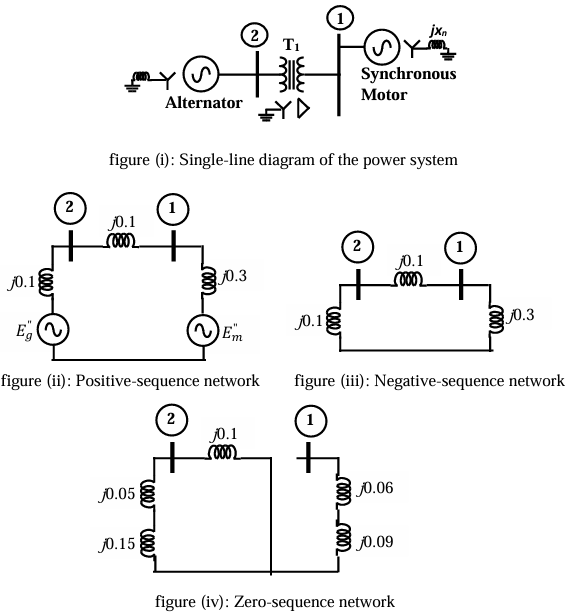
\includegraphics[width=0.7\columnwidth]{figs/Q 60.png}
    \caption{}
    \label{fig:placeholder}
\end{figure}

\item An infinite surface of linear current density $\mathbf{K} = 5\hat{a}_x$ A/m exists on the x-y plane, as shown in the figure. The magnitude of the magnetic field intensity (H) at a point (1,1,1) due to the surface current in Ampere/meter is \underline{\hspace{2cm}} (Round off to 2 decimal places).\hfill{(GATE EE 2023)}

\begin{figure}[H]
    \centering
    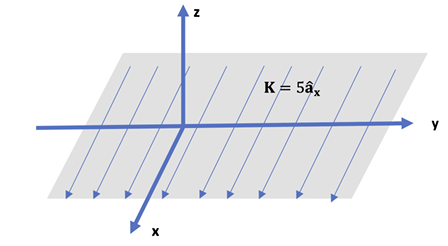
\includegraphics[width=0.5\columnwidth]{figs/Q 61.png}
    \caption{}
    \label{fig:placeholder}
\end{figure}

\item The closed curve shown in the figure is described by
$
r = 1 + \cos\theta, \quad \text{where } r = \sqrt{x^2 + y^2}; \quad x = r \cos\theta, \; y = r \sin\theta
$\\
The magnitude of the line integral of the vector field $F = -y\hat{i} + x\hat{j}$ around the closed curve is \underline{\hspace{2cm}} (Round off to 2 decimal places).\hfill{(GATE EE 2023)}
\begin{figure}[H]
    \centering
    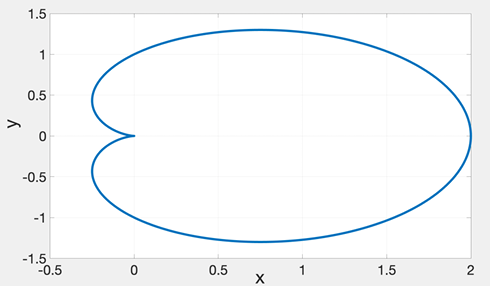
\includegraphics[width=0.5\columnwidth]{figs/Q 62.png}
    \caption{}
    \label{fig:placeholder}
\end{figure}
\item A signal $x(t) = 2\cos(180\pi t)\cos(60\pi t)$ is sampled at 200~Hz and then passed through an ideal low pass filter having cut-off frequency of 100~Hz.

The maximum frequency present in the filtered signal in Hz is \underline{\hspace{2.5cm}} (Round off to the nearest integer).\hfill{(GATE EE 2023)}

\item A balanced delta connected load consisting of the series connection of one resistor $(R = 15~\Omega)$ and a capacitor $(C = 212.21~\mu\text{F})$ in each phase is connected to three-phase, 50~Hz, 415~V supply terminals through a line having an inductance of $L = 31.83mH$ per phase, as shown in the figure. Considering the change in the supply terminal voltage with loading to be negligible, the magnitude of the voltage across the terminals $V_{AB}$ in Volts is \underline{\hspace{2.5cm}} (Round off to the nearest integer).\hfill{(GATE EE 2023)}
\begin{figure}[H]
    \centering
    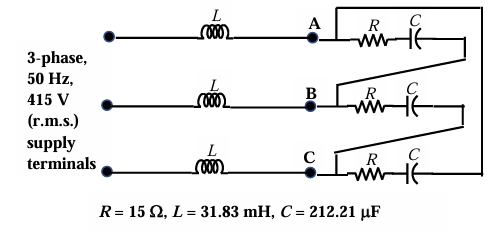
\includegraphics[width=0.8\columnwidth]{figs/Q 64.png}
    \caption{}
    \label{fig:placeholder}
\end{figure}


\item A quadratic function of two variables is given as
$
f(x_1, x_2) = x_1^2 + 2x_2^2 + 3x_1 + 3x_2 + x_1 x_2 + 1
$

The magnitude of the maximum rate of change of the function at the point $(1,1)$ is \underline{\hspace{2.5cm}} (Round off to the nearest integer).\hfill{(GATE EE 2023)}\\
\vspace{3cm}
\centering{\textbf{END OF QUESTION PAPER}}

\end{enumerate}
\end{document}









